\documentclass[10pt,twocolumn,letterpaper]{article}

% Include necessary packages
\usepackage{cvpr} % Use the review option for initial submission
\usepackage{graphicx}
\usepackage{amsmath}
\usepackage{amssymb}
\usepackage{booktabs}
\usepackage[pagebackref,breaklinks,colorlinks]{hyperref} % Enable hyperref with pagebackref
\usepackage[capitalize]{cleveref}

% Paper ID and Conference Info
\def\cvprPaperID{} % Enter the Paper ID here
\def\confName{CVPR}
\def\confYear{2022}

\begin{document}

%%%%%%%%% TITLE
\title{Food Delivery Time Prediction: Machine Learning Project}

\author{
Ananya Garg \\ \small2022068
\and Mohmmad Ayaan \\ \small2022308
\and Swara Parekh \\ \small2022524
\and Vikranth Udandarao \\ \small2022570
\and Indraprastha Institute of Information Technology, Delhi
}

\maketitle

%%%%%%%%% ABSTRACT
\begin{abstract}
    \textbf{Accurate delivery time estimates are crucial for customer satisfaction and operational efficiency in food delivery services. Delays due to traffic, weather, multiple deliveries etc. can significantly impact the customer experience. This project uses machine learning models including Linear Regression, Decision Trees, Bagging, Random Forest, XGBoost and LightGBM to predict delivery times based on data related to traffic, weather, and delivery personnel. By employing feature selection and data preprocessing, we aim to enhance prediction accuracy. Models like Random Forest and LightGBM achieve high R² scores above 0.75, demonstrating their effectiveness in improving logistics and service quality. The full project implementation is available on \href{https://github.com/Vikranth3140/Food-Delivery-Time-Prediction}{GitHub}.}
\end{abstract}

%%%%%%%%% BODY TEXT
\section{Introduction}
Running a food delivery service comes with the challenge of keeping customers happy by delivering their meals on time and in condition despite hurdles like traffic or bad weather which can throw off the schedule unpredictably.

In order to address this issue effectively we are working on a Food Delivery Time Prediction System that utilizes machine learning methods. Our goal is to predict delivery times with precision by examining delivery data, current traffic situations and real time weather trends.

%------------------------------------------------------------------------
\section{Literature Survey}
1. \textbf{DergiPark - Comparative Analysis of ML models}: The research paper titled "A Comparative Analysis of Machine Learning Models for Time Prediction in Food Delivery Operations" explores machine learning models like Random Forests and Gradient Boosting to enhance the precision of food delivery time forecasts by considering factors such as traffic volume and order quantity. Performance indicators like Mean Absolute Error (MAE) and Root Mean Square Error (RMSE) were utilized by the researchers to assess the effectiveness of these models in predicting delivery times, in real world scenarios. The results indicated that ensemble learning models, like Gradient Boosting tend to outperform methods. \cite{dergipark1}

2. \textbf{DergiPark - Application of Random Forest algorithm}: The study uses real world features to predict food delivery time. Random Forest (RF), an ensemble learning method, builds on Bagging method (combines multiple models for better accuracy) by adding randomness in feature selection, improving performance, and reducing overfitting. 500 estimator trees and three randomly selected variables per split, the model achieved around 95\% accuracy. The model struggles with imbalanced data. Cross-validation and Bootstrap methods confirmed RF's high accuracy and reliability. Performance measures like confusion matrices, Kappa statistics, and cross-validation are employed to validate the model’s accuracy and error rate. Alternative methods, like the Bootstrap method also yield high classification rates. \cite{dergipark2}

%------------------------------------------------------------------------
\section{Dataset}
    The dataset used in this project is obtained from a public source on Kaggle \cite{kaggle}. It contains records of food delivery services, with details on delivery times, weather conditions, traffic density, and information about the delivery personnel and locations involved. These features, combined with the target variable representing delivery time, make it an ideal dataset for training machine learning models to predict delivery times.

    \subsection{Data Preprocessing}
        The dataset required handling inconsistencies, mixed data types, and missing values to prepare it for machine learning, which can be viewed \href{https://github.com/Vikranth3140/Food-Delivery-Time-Prediction/blob/main/Data%20Pre%20Processing/pre-processing.py}{\textbf{here}}.

        The prefix \textit{conditions} was removed from the \textit{Weatherconditions} column. Several columns, such as \textit{ID}, \textit{Road\_traffic\_density}, \textit{Type\_of\_order}, and \textit{City}, were standardized as strings to ensure uniform data representation. The columns \textit{Delivery\_person\_Age}, \textit{Vehicle\_condition}, and \textit{multiple\_deliveries} were converted to integers, while \textit{Delivery\_person\_Ratings}, \textit{latitudes}, and \textit{longitudes} were converted to floats for further analysis. The \textit{Time\_taken(min)} was extracted and converted to integers for numerical computations.

        Additionally, the \textit{Order\_Date} column was converted to the \textit{datetime} format, and time data was extracted from both the \textit{Time\_Orderd} and \textit{Time\_Order\_picked} columns. Rows containing null values were dropped, reducing the dataset to 41,368 rows, ensuring the final dataset was clean and ready for model development.

        \subsection{Feature Summary}
        After preprocessing and standardizing, the dataset contained the following features with their respective data types:

        \begin{table}[h]
            \centering
            \begin{tabular}{|l|l|}
                \hline
                \textbf{Column Name}               & \textbf{Data Type} \\
                \hline
                ID                                 & object             \\
                Delivery\_person\_ID               & object             \\
                Delivery\_person\_Age              & int64              \\
                Delivery\_person\_Ratings          & float64            \\
                Restaurant\_latitude               & float64            \\
                Restaurant\_longitude              & float64            \\
                Delivery\_location\_latitude       & float64            \\
                Delivery\_location\_longitude      & float64            \\
                Order\_Date                        & datetime           \\
                Time\_Orderd                       & time               \\
                Time\_Order\_picked                & time               \\
                Weatherconditions                  & object             \\
                Road\_traffic\_density             & object             \\
                Vehicle\_condition                 & int64              \\
                Type\_of\_order                    & object             \\
                Type\_of\_vehicle                  & object             \\
                multiple\_deliveries               & int64              \\
                Festival                           & object             \\
                City                               & object             \\
                Time\_taken(min)                   & int64              \\
                \hline
            \end{tabular}
            \caption{Data types of the dataset features after preprocessing}
            \label{tab:dataset_dtypes}
        \end{table}

        \subsection{Exploratory Data Analysis (EDA)}
        Exploratory Data Analysis (EDA) was performed to understand the distribution of the variables in the dataset and to explore relationships between the different features. Visualizations were created to provide insights into low-key features like traffic density, weather conditions, vehicle type, and delivery person ratings that affect the time taken for deliveries.

        \begin{figure}[ht]
            \centering
            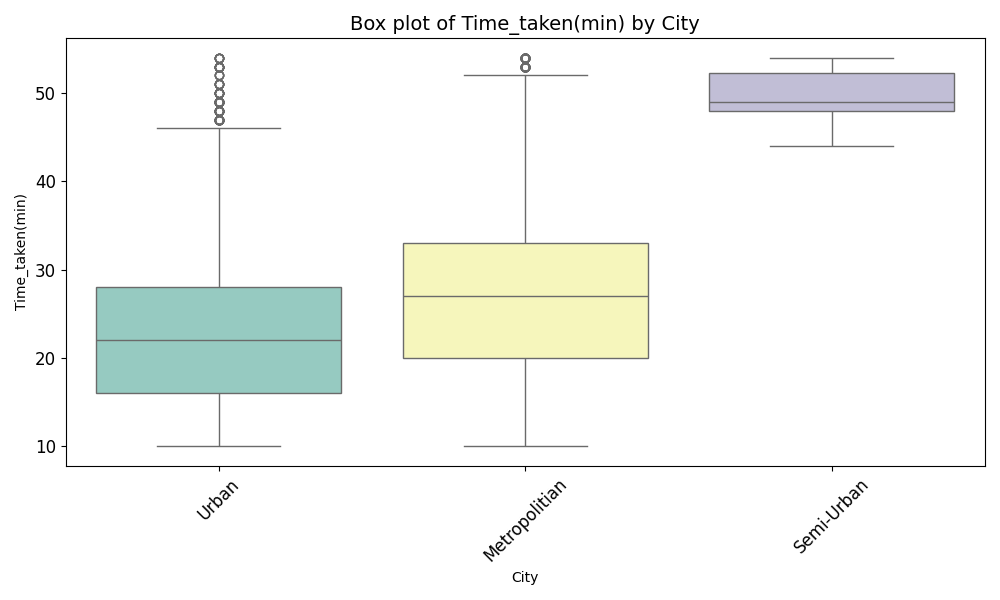
\includegraphics[width=0.45\textwidth]{boxplot_City.png}
            \caption{Time Taken (min) by City Type.}
            \label{fig:city_type}
        \end{figure}

        From the analysis, it was observed that delivery times vary significantly across different city types. Deliveries in semi-urban areas tend to take longer compared to urban and metropolitan areas. The variation in delivery times is also more pronounced in semi-urban areas, likely due to logistical challenges.

        \begin{figure}[ht]
            \centering
            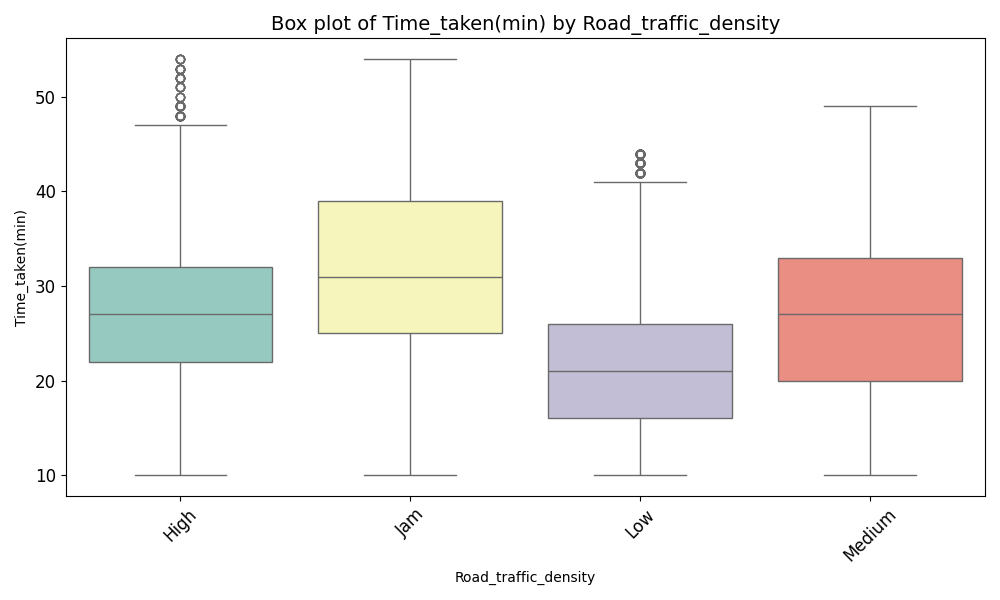
\includegraphics[width=0.45\textwidth]{boxplot_Road_traffic_density.png}
            \caption{Time Taken (min) by Road Traffic Density.}
            \label{fig:traffic_density}
        \end{figure}

        Road traffic density emerged as a key factor influencing delivery times. Areas experiencing traffic jams showed significantly longer delivery times than those with lighter traffic conditions.

        \begin{figure}[ht]
            \centering
            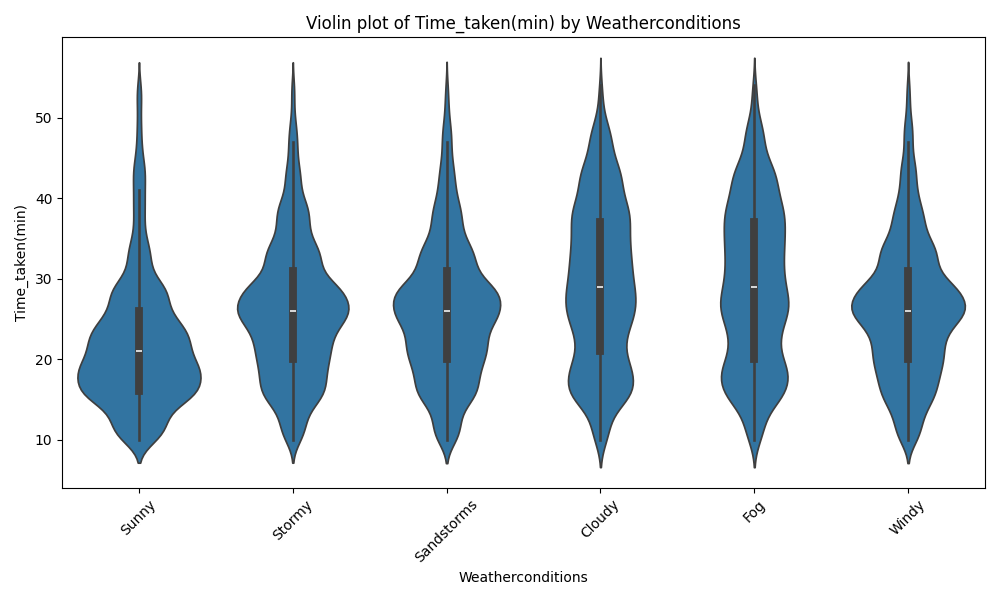
\includegraphics[width=0.45\textwidth]{violinplot_Weatherconditions.png}
            \caption{Time Taken (min) by Weather Conditions.}
            \label{fig:weather_conditions}
        \end{figure}

        Weather conditions also have a considerable effect on delivery times. Stormy, foggy, and windy conditions generally lead to longer delivery times, while sunny weather is associated with shorter delivery times, suggesting that unfavorable weather can delay deliveries.

        \begin{figure}[ht]
            \centering
            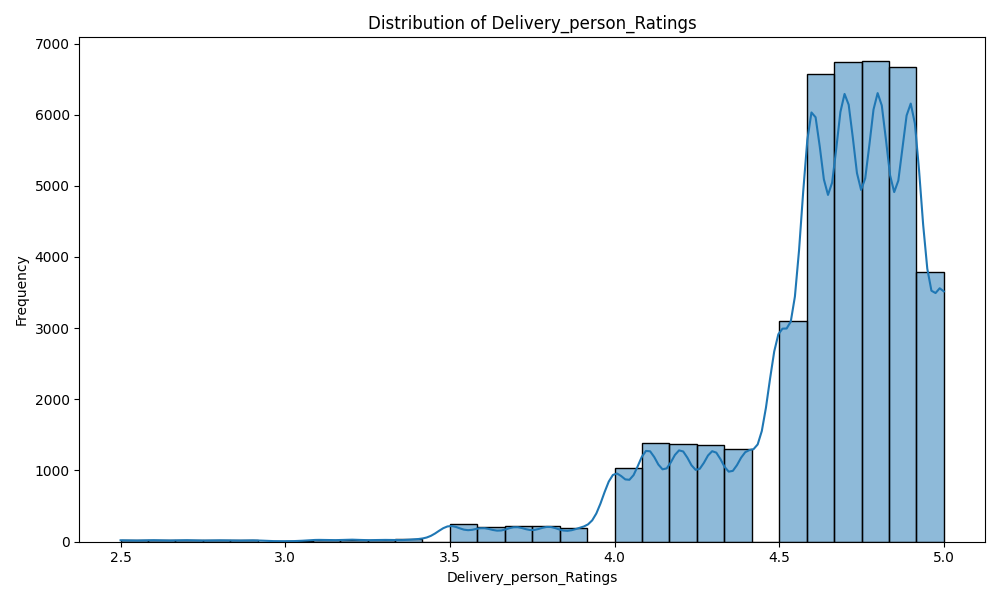
\includegraphics[width=0.45\textwidth]{histogram_Delivery_person_Ratings.png}
            \caption{Distribution of Delivery Person Ratings.}
            \label{fig:delivery_ratings}
        \end{figure}

        Analysis of delivery person ratings revealed that most delivery personnel have high ratings, with a large proportion scoring between 4.5 and 5.0, indicating a high overall level of service quality from delivery personnel.

        \begin{figure}[ht]
            \centering
            \includegraphics[width=0.7\columnwidth]{heatmap.jpg}
            \caption{Correlation HeatMap}
            \label{fig:heatmap}
        \end{figure}

        The heatmap visualizes relationships between various numeric features. Delivery Location Latitude \& Restaurant Latitude have a strong positive correlation (0.94), indicating that delivery and restaurant locations tend to align closely in latitude.

        \begin{figure}[ht]
            \centering
            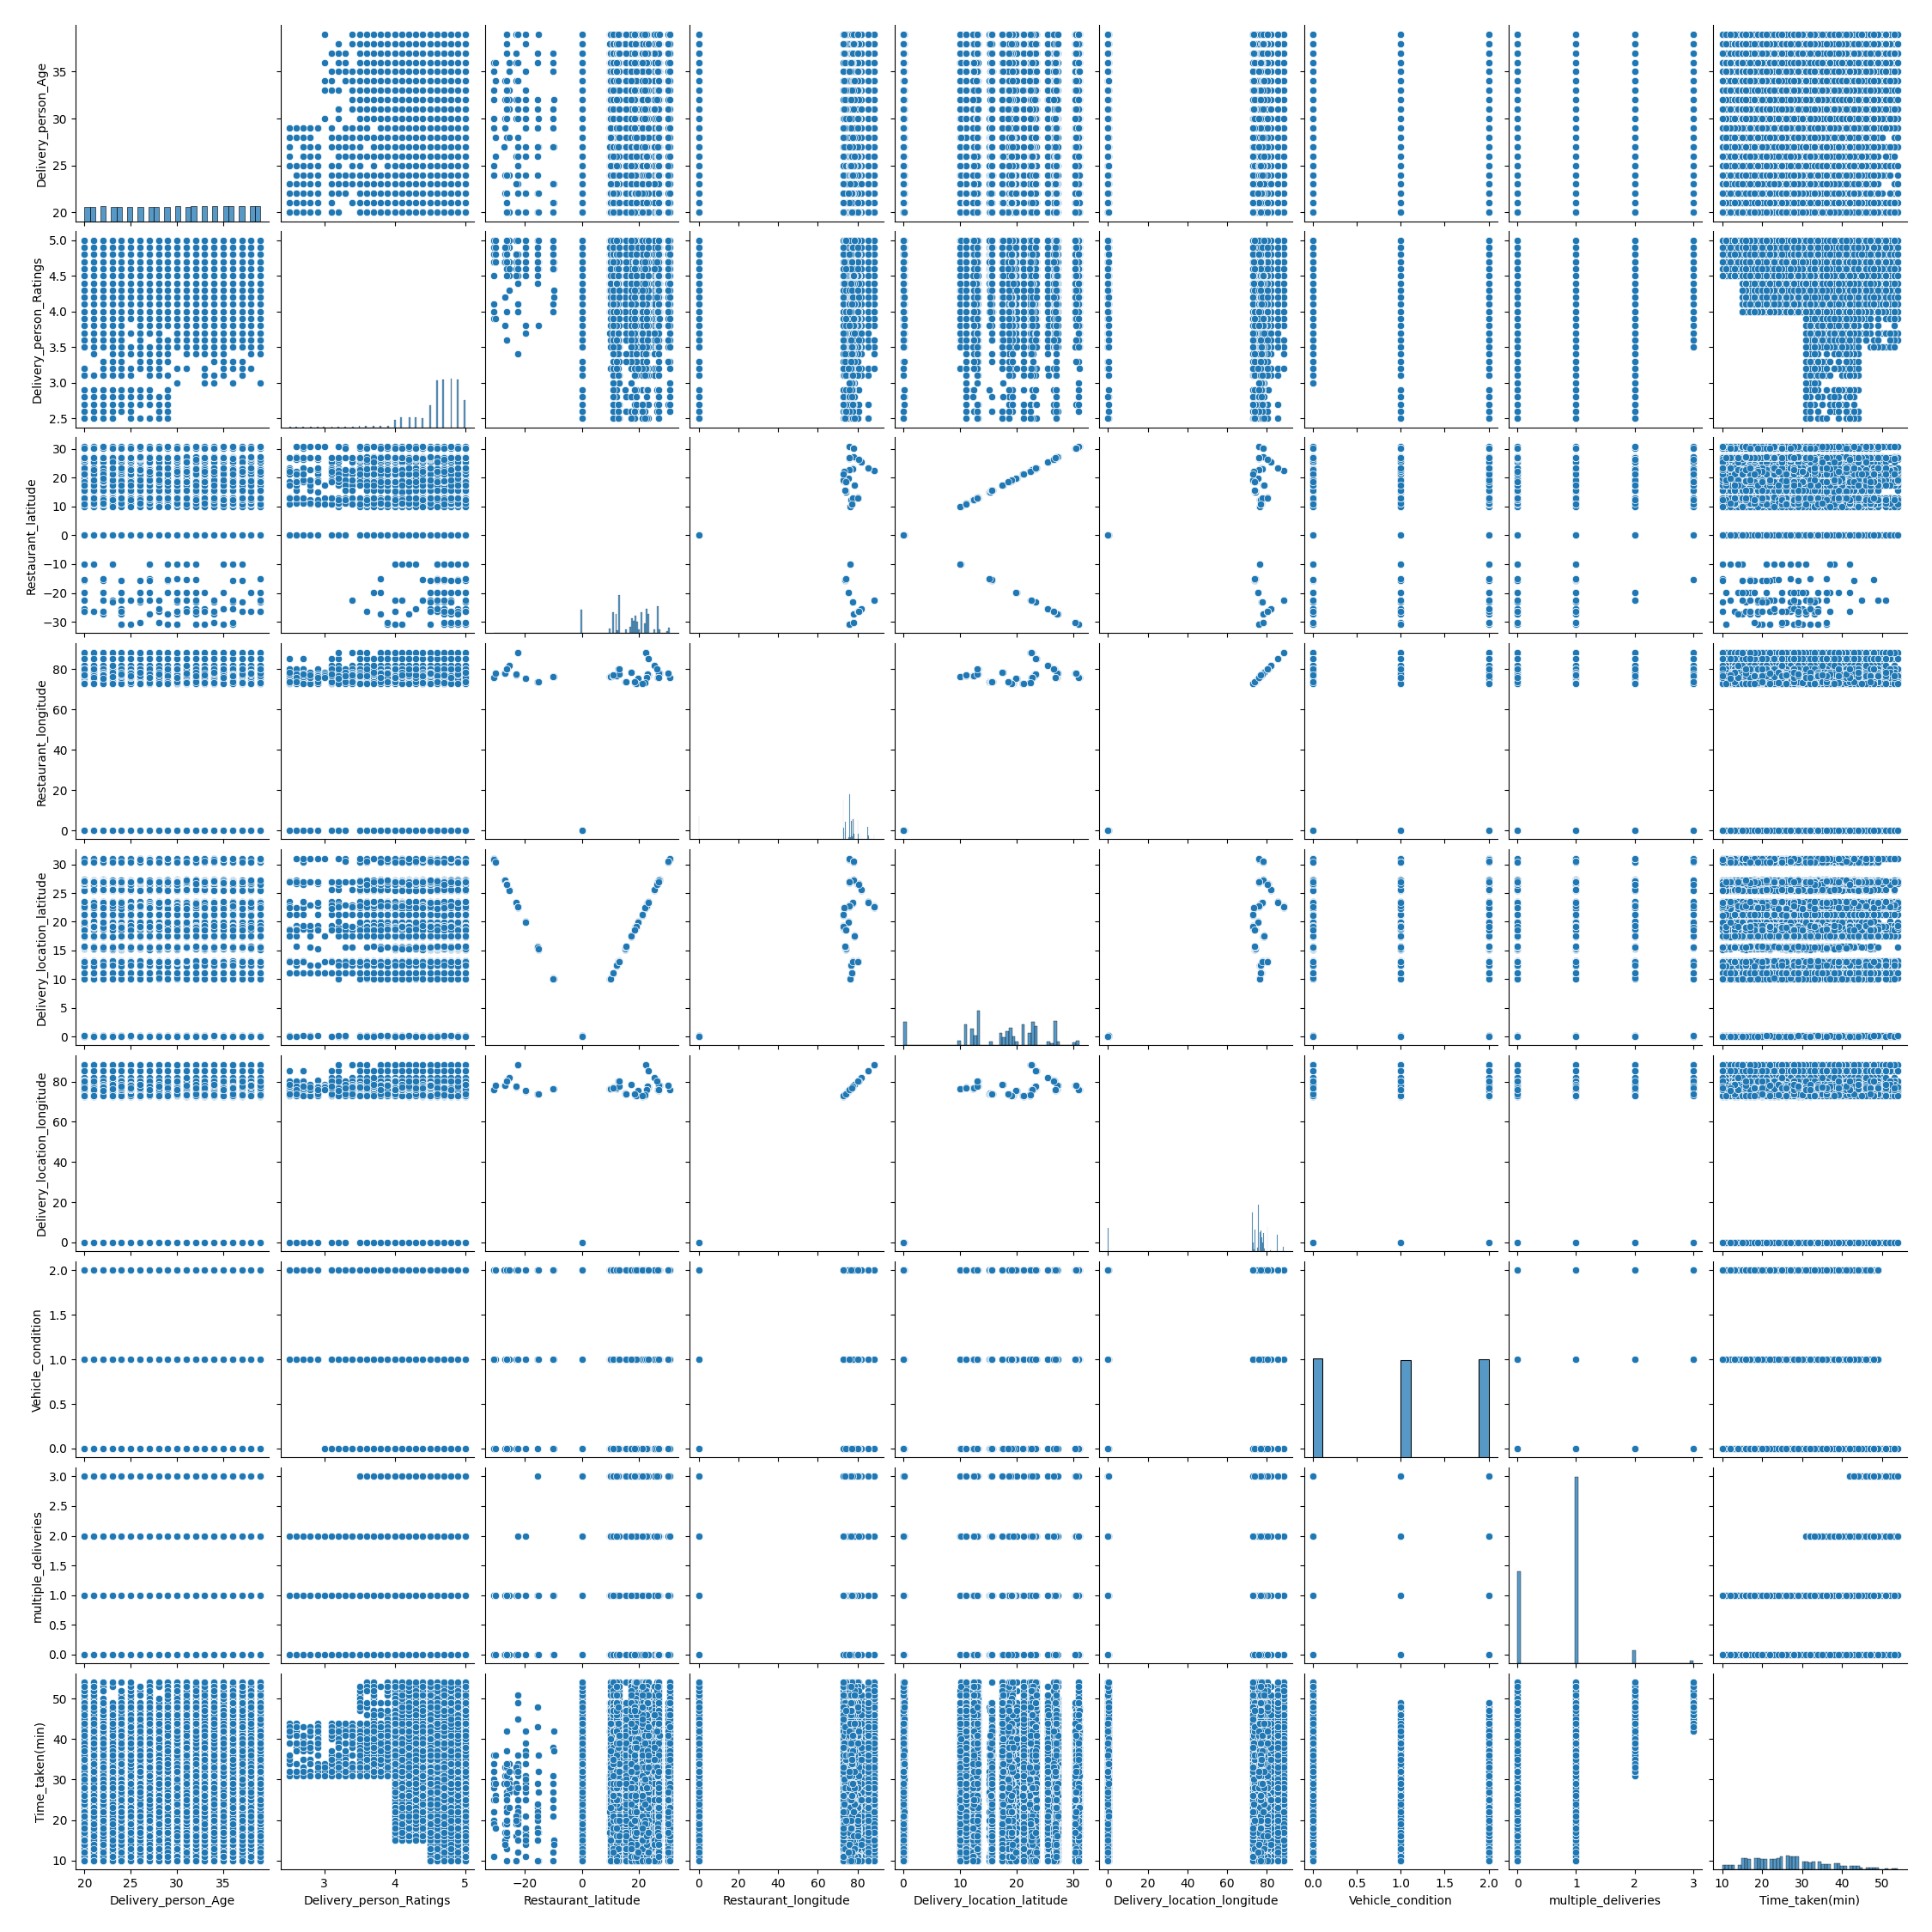
\includegraphics[width=0.7\columnwidth]{pairplot.png}
            \caption{Pair Plots for the Numerical Features}
            \label{fig:pairplot}
        \end{figure}

        Pair Plots give us the relationship between two numerical features. Delivery Location Latitude and Restaurant Latitude exhibit a clear linear trend suggesting a strong geographical alignment between delivery and restaurant locations, indicating faster deliveries.

        Overall, the EDA identified key variables influencing delivery time, such as traffic density, weather conditions, city type, and vehicle type. These factors are important for building predictive models for delivery time estimation.

%------------------------------------------------------------------------
\section{Methodology}
    The main objective is to predict food delivery times using machine learning techniques. The dataset contains 19 different features that determine the prediction.

    We followed a structured methodology which involved the following steps:
    \begin{itemize}
        \item \textbf{Data Collection and Preprocessing}: The dataset was preprocessed to handle inconsistencies, missing values, and data types while categorical variables were label-encoded.
        
        \item \textbf{Exploratory Data Analysis (EDA)}: Visualizations such as box plots, violin plots, pair plots, correlation heatmap and Umap were generated to understand feature distributions and relationships.
        
        \item \textbf{Feature Selection}: The k-best feature selection method was applied to identify the most relevant predictors for delivery time. Key features such as \textit{Road\_traffic\_density}, \textit{Festival}, \textit{multiple\_deliveries}, \textit{Delivery\_person\_Ratings}, \textit{Delivery\_person\_Age}, \textit{City}, \textit{Weatherconditions}, \textit{Vehicle\_condition}, and \textit{Type\_of\_vehicle} were selected, improving model efficiency and reducing the risk of overfitting.
        % \item \textbf{Feature Selection}: Feature importance techniques, such as using Random Forest's feature importances, were employed to identify the most influential features.
        \item \textbf{Model Training and Evaluation}: Multiple machine learning models were trained, evaluated, and compared using performance metrics such as R² score and Mean Squared Error (MSE).
    
    \end{itemize}
    
    \subsection{Model Selection}
        For predicting food delivery times, we explored regression techniques and ensemble methods like Linear Regression, Decision Trees, Bagging, Random Forests, Elastic Net Regularization, LightGBM, XGBoosting, and K-fold cross-validation.

        \subsubsection{Linear Regression}
            It assumes a linear correlation between input features and the target variable was applied to explore the dataset’s linear relationships. Although it provided initial insights, the relatively high MSE indicates that the model's predictions have considerable errors, and its performance is limited due to the complex nature of the data.

        \subsubsection{Decision Tree}
            DTs use structures to represent decisions. The MSE indicates that the model's predictions deviate significantly from the actual delivery times, suggesting it leads to overfitting on testing data, leading to poor performance.

        \subsubsection{Bagging}
            It improves model performance by training multiple models on random subsets of the original data. The MSE indicates a reasonable level of accuracy in predicting delivery times, while the R² score suggests a fair result.

        \subsubsection{Random Forest}
            It is utilized as an ensemble learning method to construct multiple decision trees during training and merge their outputs. The relatively low MSE indicates that the model performs well in predicting delivery times, while the R² score again suggests a fair result.

        \subsubsection{Elastic Net Regularization}
            It combines L1 and L2 regularization to handle multicollinearity and perform feature selection. The relatively high MSE and low R² score indicate that the model has significant prediction errors, suggesting poor accuracy.

        \subsubsection{LightGBM}
            LightGBM splits trees leaf-wise, rather than level-wise.
            The low MSE indicates that the model provides accurate predictions of delivery times, while the R² score suggests a decrease in overfitting and a better result overall.

        \subsubsection{XGBoost}
            XGBoost an ensemble learning that iteratively builds a predictive model by combining predictions from multiple individual models. The relatively low MSE and the R² score indicate that the model produces accurate predictions of delivery times and is effective in capturing complex patterns in the data.

        \subsubsection{K-Fold Cross-Validation}
            The model is trained on K-1 folds and tested on the remaining folds. This process is repeated K times, using each fold as the validation set. The Average Silhouette Score (a measure of how similar an object is to its own cluster compared to other) obtained from K-Fold Cross-Validation was 0.2889, indicating a moderate level of clustering quality.

        \subsubsection{SVM}
            Support Vector Machines work by finding the optimal hyperplane in a high-dimensional space. The relatively low accuracy suggests inefficiency in capturing the complex patterns in the data, due to high-dimensional feature space or non-linear relationships.

%------------------------------------------------------------------------
\section{Results and Analysis}

    \begin{table}[h!]
        \centering
        % \caption{Test Metrics for Different Models}
        \begin{tabular}{|l|l|l|}
            \hline
            \textbf{Model} & \textbf{MSE} & \textbf{R² Score} \\ \hline
            Linear Regression              & 49.08     & 0.44      \\ \hline
            Decision Tree                  & 43.09     & 0.51      \\ \hline
            Decision Tree with Bagging     & 30.28     & 0.65     \\ \hline
            Random Forest                  & 30.03     & 0.66      \\ \hline
            Elastic Net Regularization     & 57.36     & 0.34      \\ \hline
            LightGBM                      & 20.59    & 0.76     \\ \hline
            XGBoost                       & 25.37     & 0.71      \\ \hline
            SVM                       & 34.47     & 0.61      \\ \hline
        \end{tabular}
        \label{tab:model_metrics}
    \end{table}

    The table above presents the test metrics for various machine learning models, using Mean Squared Error (MSE) and R² Score. LightGBM achieved the highest R² Score (0.76) and the lowest MSE (20.59), followed closely by XGBoost and Random Forest, both with R² Scores around 0.65. Bagging also demonstrated improvement over a standalone Decision Tree model, highlighting the effectiveness of ensemble methods. In contrast, Linear Regression and Elastic Net Regularization showed lower predictive performance, indicating complex models are preferable.

%------------------------------------------------------------------------
\section{Conclusion}
    The aim was to predict food delivery times by analyzing key variables, including traffic density, delivery volume, location specifics, order types, vehicle conditions, and delivery personnel ratings.

    Following data preprocessing and exploratory data analysis, various regression and ensemble methods were evaluated to build the prediction model.

    A user-friendly CLI has been implemented, allowing users to input feature values and obtain predicted delivery times. The predictions are generated using the LightGBM model, since it gained the most accuracy.

    \subsection{Individual Contribution}
        - \textbf{Vikranth Udandarao}: Literature review, Data Collection, EDA, dataset visualization, model analysis and results.

        - \textbf{Swara Parekh}: Literature review, Data Collection, EDA, visualization of dataset, model analysis and results.

        - \textbf{Mohmmad Ayaan}: Literature review, Data Collection, EDA, visualization of dataset, model analysis and results.

        - \textbf{Ananya Garg}: Literature review, Data Collection, EDA, visualization of dataset, model analysis and results.

\newpage

%%%%%%%%% REFERENCES
\begin{thebibliography}{9}
    
    \bibitem{dergipark1}
        Comparative Analysis of ML Models for Food Delivery Prediction.
        Available at: \url{https://dergipark.org.tr/en/pub/aita/issue/84471/1459560}.
    
    \bibitem{dergipark2}
        Application of Random Forest Algorithm in Food Delivery Time Prediction.
        Available at: \url{https://dergipark.org.tr/en/pub/forecasting/issue/60291/842180}.
    
    \bibitem{kaggle}
        Gaurav Malik.
        \emph{Food Delivery Dataset}.
        Available at: \url{https://www.kaggle.com/datasets/gauravmalik26/food-delivery-dataset/data}.
    
    \bibitem{scikit-learn}
        Pedregosa, F., Varoquaux, G., Gramfort, A., Michel, V., Thirion, B., Grisel, O., Blondel, M., Prettenhofer, P., Weiss, R., Dubourg, V., Vanderplas, J., Passos, A., Cournapeau, D., Brucher, M., Perrot, M., Duchesnay, E.
        \emph{Scikit-learn: Machine Learning in Python}.
        Journal of Machine Learning Research, 12, pp. 2825-2830, 2011.
        Available at: \url{https://scikit-learn.org}.
    
    \bibitem{lightgbm}
        Ke, G., Meng, Q., Finley, T., Wang, T., Chen, W., Ma, W., Ye, Q., and Liu, T. Y.
        \emph{LightGBM: A Highly Efficient Gradient Boosting Decision Tree}.
        Advances in Neural Information Processing Systems 30 (NIPS 2017).
        Available at: \url{https://lightgbm.readthedocs.io}.
    
    \bibitem{xgboost}
        Chen, T. and Guestrin, C.
        \emph{XGBoost: A Scalable Tree Boosting System}.
        Proceedings of the 22nd ACM SIGKDD International Conference on Knowledge Discovery and Data Mining, 2016.
        Available at: \url{https://xgboost.readthedocs.io}.
    
\end{thebibliography}

\end{document}